\documentclass[189]{pset}

% ================================================================== %
%                                                                    %
%                              Document                              %
%                                                                    %
% ================================================================== %

% ----------------------- Header formatting ------------------------ %

\name{Forest Kobayashi}
\class{Math of Big Data}
\season{Summer}
\prof{Gu}
\assignment{1}
\duedate{05/15/2018}
\dueday{Tuesday}
\problems{1, 2}
\acknowledgements{{Tim Player, Jacky Lee}, {}}
\onTime{0}

\comments{\textbf{Comments}: Feel free to work with other students,
  but make sure you write up the homework and code on your own (no
  copying homework \textit{or} code; no pair programming). Feel free
  to ask students or instructors for help debugging code or whatever
  else, though.

  The starter code for problem 2 part c and d can be found under the
  Resource tab on course website.

  \textit{Note:} You need to create a Github account for submission of
  the coding part of the homework. Please create a repository on
  Github to hold all your code and include your Github account
  username as part of the answer to problem 2.}

\lfoot{Due Tuesday, May 15th 2018}

\newenvironment{amatrix}[1]{%
  \left[\begin{array}{@{}*{#1}{c}|c@{}}
}{%
  \end{array}\right]
}

\begin{document}

% --------------------------- Problem 1 ---------------------------- %

  \section{(Linear Transformation)}
    Let $\vy = A \vx + \vb$ be a random vector. Show that
    expectation is linear:
    \[
      \EE[\vy] = \EE[A\vx + \vb] = A\EE[\vx] + \vb.
    \]
    Also show that
    \[
      \cov[\vy] = \cov[A\vx + \vb] = A \cov[\vx] A^\T = A\mb\Sigma A^\T.
    \]

  \hrulefill

  \section*{Solution:}
    \begin{enumerate}
      \item First, we prove some small lemmas.
        \begin{lemma}
          Let $X$ be a continuous random variable, and $a$ be a
          scalar. Then $\EE\bk{aX}=a\EE\bk{X}$.
        \end{lemma}
        \begin{proof}
          Let $X$ admit a density function $f(x)$. Then
          \begin{align*}
            \EE\bk{aX}
            &= \int_{-\infty}^\infty axf(x) \dd x \\
            &= a\int_{-\infty}^\infty xf(x) \dd x \\
            &= a\EE\bk{X}
          \end{align*}
        \end{proof}
        \begin{lemma}
          Let $X$ be a random variable, and let $a$ be a scalar. Then
          $\EE\bk{X+a}=\EE\bk{X}+\EE\bk{a}=\EE\bk{X}+a$.
        \end{lemma}
        \begin{proof}
          Let $X$ admit a density function $f(x)$. Then over $\RR$,
          $f(x)$ must integrate to 1. Hence
          \begin{align*}
            \int_{-\infty}^\infty (x+a)f(x) \dd x
            &= \int_{-\infty}^\infty xf(x) + af(x) \dd x \\
            &= \int_{-\infty}^\infty xf(x) \dd x +
              \int_{-\infty}^\infty af(x) \dd x \\
            &= \int_{-\infty}^\infty xf(x) \dd x +
              a\int_{-\infty}^\infty f(x) \dd x \\
            &= \EE\bk{X} + a\cdot 1 \\
            &= \EE\bk{X} + a
          \end{align*}
        \end{proof}
        \begin{lemma}
          Let $X$ and $Y$ be continuous random variables. Then
          $\EE\bk{X+Y} = \EE\bk{X}+\EE\bk{Y}$.
        \end{lemma}
        \begin{proof}
          Let $X+Y$ have a density function $f(x,y)$. Then
          \begin{align*}
            \EE\bk{X+Y}
            &= \int_{-\infty}^\infty \int_{-\infty}^\infty
              (x+y)f(x,y)\dd x \dd y \\
            &= \int_{-\infty}^\infty \int_{-\infty}^\infty xf(x,y) \dd
              x \dd y + \int_{-\infty}^\infty \int_{-\infty}^\infty
              yf(x,y) \dd x \dd y \\
            &= \EE\bk{X} + \EE\bk{Y}
          \end{align*}
        \end{proof}
        Now we do the main problem. By the lemmas, we have
        \begin{align*}
          \EE\bk{\vy}
          &= \EE\bk{A\vx + \vb} \\
          &= \EE\bk{A\vx} + \EE\bk{\vb} \\
          &= \EE\bk{A\vx} + \vb
        \end{align*}
        It remains to show that $\EE\bk{A\vx} = A\EE\bk{\vx}$. Suppose
        $\vx$ is an $n$-dimensional random vector in a space $X$:
        \[
          \vx =
          \begin{bmatrix}
            x_0 \\
            x_1 \\
            \vdots \\
            x_n
          \end{bmatrix}
        \]
        where each of the $x_i \in \RR$. By definition, the
        expectation value of $\vx$ is given by
        \[
          \EE\bk{\vx} =
          \begin{bmatrix}
            \EE\bk{x_0} \\
            \EE\bk{x_1} \\
            \vdots \\
            \EE\bk{x_n}
          \end{bmatrix}
        \]
        % and for any continuous random variable, we have
        % \[
        %   \EE\bk{Y} = \int_{-\infty}^\infty y f(y) \dd y
        % \]
        % where $f(y)$ is some probability density function. For each of
        % the $x_i$, define $f_i(x_i)$ to be the corresponding
        % probability density function. Then
        % \begin{align*}
        %   \EE\bk{\vx}
        %   &=
        %     \begin{bmatrix}
        %       \displaystyle\int_{-\infty}^\infty x_0 f_0(x_0) \dd x_0
        %       \\[1em]
        %       \displaystyle\int_{-\infty}^\infty x_1 f_1(x_1) \dd x_1
        %       \\[1em]
        %       \vdots \\[1em]
        %       \displaystyle\int_{-\infty}^\infty x_n f_n(x_n) \dd x_n
        %     \end{bmatrix}
        % \end{align*}
        Let $A \in M_{m\times n}(\RR)$, with rows $\va_0$, $\va_1$,
        $\ldots$, $\va_m$. Then $A\EE\bk{\vx}$ is given by
        \begin{align*}
          A\EE\bk{\vx}
          &=
            \begin{bmatrix}
              a_{0,0} & a_{0,1} & \cdots & a_{0,n} \\
              a_{1,0} & a_{1,1} & \cdots & a_{1,n} \\
              \vdots & \vdots & \ddots & \vdots \\
              a_{m,0} & a_{m,1} & \cdots & a_{m,n}
            \end{bmatrix}
            \begin{bmatrix}
              \EE\bk{x_0} \\
              \EE\bk{x_1} \\
              \vdots \\
              \EE\bk{x_n}
            \end{bmatrix} \\
          &=
            \begin{bmatrix}
              \displaystyle\sum_{i=0}^n a_{0,i}\EE\bk{x_i} \\[1em]
              \displaystyle\sum_{i=0}^n a_{1,i}\EE\bk{x_i} \\[1em]
              \vdots\\
              \displaystyle\sum_{i=0}^n a_{n,i}\EE\bk{x_i}
            \end{bmatrix}
        \end{align*}
        Now, we manipulate this expression to obtain $\EE\bk{A\vx}$.
        Because the expected value of a sum is the sum of expected
        values (see lemmas), we have
        \begin{align*}
          \begin{bmatrix}
            \displaystyle\sum_{i=0}^n a_{0,i}\EE\bk{x_i} \\[1em]
            \displaystyle\sum_{i=0}^n a_{1,i}\EE\bk{x_i} \\[1em]
            \vdots\\
            \displaystyle\sum_{i=0}^n a_{n,i}\EE\bk{x_i}
          \end{bmatrix}
          &=
            \begin{bmatrix}
              \displaystyle\EE\bk{\sum_{i=0}^n a_{0,i}x_i} \\[1.5em]
              \displaystyle\EE\bk{\sum_{i=0}^n a_{1,i}x_i} \\[1.5em]
              \vdots\\
              \displaystyle\EE\bk{\sum_{i=0}^n a_{n,i}x_i}
            \end{bmatrix}
          \shortintertext{and now because the expected value of a
          vector is a vector of expected values,}
          \begin{bmatrix}
            \displaystyle\EE\bk{\sum_{i=0}^n a_{0,i}x_i} \\[1.5em]
            \displaystyle\EE\bk{\sum_{i=0}^n a_{1,i}x_i} \\[1.5em]
            \vdots\\
            \displaystyle\EE\bk{\sum_{i=0}^n a_{n,i}x_i}
          \end{bmatrix}
          &= \EE\bk{
            \begin{bmatrix}
              \displaystyle \sum_{i=0}^n a_{0,i} x_i \\[1em]
              \displaystyle \sum_{i=0}^n a_{1,i} x_i \\[1em]
              \vdots \\
              \displaystyle \sum_{i=0}^n a_{m,i} x_i
            \end{bmatrix}
          } \\
          &= \EE\bk{A\vx}
        \end{align*}
        hence $A\EE\bk{\vx} = \EE\bk{A\vx}$, and so putting all the
        pieces together,
        \[
          \boxed{\EE\bk{A\vx + \vb} = A\EE\bk{\vx} + \vb}
        \]
        as desired. \qed
      \item We have the following corollary to part (a):
        \begin{corollary}
          Let $A$ be a matrix, and let $\vx$ be a random vector. Then
          $\EE\bk{\vx A^\T} = \EE\bk{\vx}A^\T$.
        \end{corollary}
        \begin{proof}
          Note that
          \begin{align*}
            \EE\bk{\vx A^\T}
            &= \EE\bk{\pn{\pn{\vx A^\T}^\T}^\T} \\
            &= \EE\bk{\pn{A \vx^\T}^\T} \\
            &= \pn{\EE\bk{A\vx^\T}}^\T \\
            &= \pn{A\EE\bk{\vx^\T}}^\T \\
            &= \pn{\EE\bk{\vx^\T}}^\T A^\T \\
            &= \EE\bk{\vx} A^\T
          \end{align*}
        \end{proof}
        Now, we proceed to the main proof. The covariance matrix
        $\cov\bk{\vy}$ is defined by
        \begin{align*}
          \cov\bk{\vy}
          &=
            \begin{bmatrix}
              \EE\bk[Big]{\pn{y_0 - \EE\bk{y_0}}\pn{y_0 - \EE\bk{y_0}}}
              & \EE\bk[Big]{\pn{y_0 - \EE\bk{y_0}}\pn{y_1 - \EE\bk{y_1}}}
              & \cdots
              & \EE\bk[Big]{\pn{y_0 - \EE\bk{y_0}}\pn{y_n - \EE\bk{y_n}}}
              \\[1em]
              \EE\bk[Big]{\pn{y_1 - \EE\bk{y_1}}\pn{y_0 - \EE\bk{y_0}}}
              & \EE\bk[Big]{\pn{y_1 - \EE\bk{y_1}}\pn{y_1 - \EE\bk{y_1}}}
              & \cdots
              & \EE\bk[Big]{\pn{y_1 - \EE\bk{y_1}}\pn{y_n - \EE\bk{y_n}}}
              \\[1em]
              \vdots & \vdots & \ddots & \vdots \\[1em]
              \EE\bk[Big]{\pn{y_n - \EE\bk{y_n}}\pn{y_0 - \EE\bk{y_0}}}
              & \EE\bk[Big]{\pn{y_n - \EE\bk{y_n}}\pn{y_1 - \EE\bk{y_1}}}
              & \cdots
              & \EE\bk[Big]{\pn{y_n - \EE\bk{y_n}}\pn{y_n - \EE\bk{y_n}}}
            \end{bmatrix} \\
          &=
            \begin{bmatrix}
              \cov\pn{y_0,y_0} & \cov\pn{y_0,y_1} & \cdots &
              \cov\pn{y_0, y_n} \\
              \cov\pn{y_1,y_0} & \cov\pn{y_1,y_1} & \cdots &
              \cov\pn{y_1, y_n} \\
              \vdots & \vdots & \ddots & \vdots \\
              \cov\pn{y_n, y_0} & \cov\pn{y_n, y_1} & \cdots &
              \cov\pn{y_n, y_n}
            \end{bmatrix}
        \end{align*}
        it is a property of covariance that for all random variables
        $X$ and $Y$, with scalars $a$ and $b$, $\cov\pn{X+a,Y+b} =
        \cov\pn{X,Y}$. Hence, since each $y_i = (A\vx)_i + b_i$, then
        $\forall i,j \in \set{0,1,\ldots,n}$,
        \begin{align*}
          \cov\bk{y_i,y_j}
          &= \cov\bk{(A\vx)_i + b_i, (A\vx)_j + b_j} \\
          &= \cov\bk{(A\vx)_i, (A\vx)_j}
        \end{align*}
        thus, examining the matrix above, we see $\cov\bk{A\vx + \vb}
        = \cov\bk{A\vx}$. It remains to show $\cov{\bk{A\vx}} =
        A\cov\bk{\vx}A^\top$.

        Note that we can reexpress the covariance matrix by
        \begin{align*}
          \cov\bk{y}
          &=
            \EE\bk{
            \begin{bmatrix}
              (y_0-\EE\bk{y_0})(y_0-\EE\bk{y_0})
              & (y_0-\EE\bk{y_0})(y_1-\EE\bk{y_1})
              & \cdots
              & (y_0-\EE\bk{y_0})(y_n-\EE\bk{y_n}) \\[1em]
              (y_1-\EE\bk{y_1})(y_0-\EE\bk{y_0})
              & (y_1-\EE\bk{y_1})(y_1-\EE\bk{y_1})
              &\cdots
              & (y_1-\EE\bk{y_1})(y_n-\EE\bk{y_n}) \\[1em]
              \vdots & \vdots & \ddots & \vdots \\[1em]
              (y_n-\EE\bk{y_n})(y_0-\EE\bk{y_0})
              & (y_n-\EE\bk{y_n})(y_1-\EE\bk{y_1})
              & \cdots
              & (y_n-\EE\bk{y_n})(y_n-\EE\bk{y_n})
            \end{bmatrix}
                }\\
          &= \EE\bk{(\vy - \EE\bk{\vy})(\vy-\EE\bk{\vy})^\T} \\
          &= \EE\bk{(A\vx - \EE\bk{A\vx})(A\vx-\EE\bk{A\vx})^\T}
            \shortintertext{by part (a),}
          &= \EE\bk{(A\vx - A\EE\bk{\vx})(A\vx - A\EE\bk{\vx})^\T}\\
          &= \EE\bk{(A\vx - A\EE\bk{\vx})(\vx^\T A^\T - \EE\bk{\vx}^\T
            A^\T)} \\
          &= \EE\bk{A\pn{\vx- \EE\bk{\vx}}(\vx^\T - \EE\bk{\vx}^\T)
            A^\T}\\
          &= \EE\bk{A\pn{\vx- \EE\bk{\vx}}(\vx-\EE\bk{\vx})^\T
            A^\T}\\
          % &= \EE\bk{A\vx\vx^\T A^\T - A\vx\EE\bk{\vx}^\T A^\T
          %   -A\EE\bk{\vx}\vx^\T A^\T + A\EE\bk{\vx}\EE\bk{\vx}^\T
          %   A^\T} \\
          % &= \EE\bk{A\pn{\vx \vx^\T - \vx \EE\bk{\vx}^\T -
          %   \EE\bk{\vx}\vx^\T + \EE\bk{\vx}\EE\bk{\vx}^\T}A^\T} \\
          % &= A\EE\bk{\pn{\vx \vx^\T - \vx \EE\bk{\vx}^\T -
          %   \EE\bk{\vx}\vx^\T + \EE\bk{\vx}\EE\bk{\vx}^\T}A^\T} \\
          % &= A\EE\bk{\pn{\vx \vx^\T - \vx \EE\bk{\vx}^\T -
          %   \EE\bk{\vx}\vx^\T + \EE\bk{\vx}\EE\bk{\vx}^\T}}A^\T \\
          &= A\EE\bk{\pn{\vx - \EE\bk{\vx}}\pn{\vx - \EE\bk{\vx}}^\T}
            A^\T \\
          &= A\cov\bk{\vx} A^\T = A \bm{\Sigma} A^\T
        \end{align*}
        hence, putting it all together, we have
        \[
          \boxed{\cov\bk{A\vx + \vb} = A\cov\bk{\vx}A^\T}
        \]
        \qed
    \end{enumerate}
  \clearpage

% --------------------------- Problem 2 ---------------------------- %

  \section{}
    Given the dataset $\cD = \{(x,y)\} = \{(0,1), (2,3), (3,6), (4,8)\}$
    \begin{enumerate}
      \item Find the least squares estimate $y = {\bm{\theta}}^\T\vx$ by
        hand using Cramer's Rule.
      \item Use the normal equations to find the same solution and
        verify it is the same as part (a).
      \item Plot the data and the optimal linear fit you found.
      \item Find randomly generate 100 points near the line with white
        Gaussian noise and then compute the least squares estimate
        (using a computer). Verify that this new line is close to the
        original and plot the new dataset, the old line, and the new
        line.
    \end{enumerate}

  \hrulefill

  \section*{Solution:}
  My github username is \texttt{redpanda1234}.
  \begin{enumerate}
    \item By Cramer's rule, we have
      \begin{align*}
        m
        &= \frac{\displaystyle n \sum_{i=1}^n \bk{x_iy_i} -
          \pn{\sum_{i=1}^n x_i}\pn{\sum_{i=1}^n y_i}}{\displaystyle n
          \sum_{i=1}^n \bk{x_i^2} - \pn{\sum_{i=1}^n x_i}^2} \\
        &= \frac{4\pn{0+6+18+32} -
          \pn{0+2+3+4}\pn{1+3+6+8}}{4\pn{0+4+9+16} - \pn{0+2+3+4}^2}
        \\
        &= \frac{4\pn{56} - \pn{9\cdot 8}}{4\pn{29} - 9^2} \\
        &= \frac{224 - 162}{116 - 81} \\
        &= \boxed{\frac{62}{35}}
      \end{align*}
      and
      \begin{align*}
        b
        &= \frac{\displaystyle \pn{\sum_{i=1}^n x_i^2}\pn{\sum_{i=1}^n
          y_i} - \pn{\sum_{i=1}^n x_i}\pn{\sum_{i=1}^n x_iy_i}}{
          \displaystyle n \sum_{i=1}^n \bk{x_i^2} - \pn{\sum_{i=1}^n
          x_i}^2} \\
        &= \frac{\pn{0 + 4 + 9 + 16}\pn{1 + 3 + 6 +8} - \pn{0 + 2 + 3
          + 4}\pn{0 + 6 + 18 + 32}}{35} \\
        &= \frac{29\cdot 18 - 9\cdot 56}{35} \\
        &= \frac{522 - 504}{35} \\
        &= \boxed{\frac{18}{35}}
      \end{align*}
    \item By the normal equation,
      \[
        X^\T \vy = X^\T X \bm{\theta}
      \]
      we have
      \[
        X =
        \begin{bmatrix}
          1 & 0 \\
          1 & 2 \\
          1 & 3 \\
          1 & 4
        \end{bmatrix}
        \qquad
        \vy =
        \begin{bmatrix}
          1 \\
          3 \\
          6 \\
          8
        \end{bmatrix}
      \]
      thus
      \begin{align*}
        X^\T X
        &=
          \begin{bmatrix}
            4 & 9 \\
            9 & 29
          \end{bmatrix}
      \end{align*}
      and
      \[
        X^\T \vy =
        \begin{bmatrix}
          18 \\
          56
        \end{bmatrix}
      \]
      hence
      \begin{align*}
        \begin{bmatrix}
          18 \\
          56
        \end{bmatrix}
        &=
          \begin{bmatrix}
            4 & 9 \\
            9 & 29
          \end{bmatrix}
                \begin{bmatrix}
                  \theta_0 \\
                  \theta_1
                \end{bmatrix}
      \end{align*}
      so we solve the following:
      \begin{align*}
        \begin{amatrix}{2}
          4 & 9 & 18 \\
          9 & 29 & 56
        \end{amatrix} \\
        \begin{amatrix}{2}
          4 & 9 & 18 \\
          1 & 11 & 20
        \end{amatrix} \\
        \begin{amatrix}{2}
          0 & -35 & -62 \\
          1 & \ph 11 & 20
        \end{amatrix}\\
        \begin{amatrix}{2}
          0 & 1 & \frac{62}{35} \\[.5em]
          1 & 11 & 20
        \end{amatrix}\\
        \begin{amatrix}{2}
          0 & 1 & \frac{62}{35} \\[.5em]
          1 & 0 & \frac{18}{35}
        \end{amatrix}
      \end{align*}
      thus
      \[
        \bm{\theta} =
        \begin{bmatrix}
          b \\
          m
        \end{bmatrix}
        =
        \begin{bmatrix}
          \frac{62}{35} \\[.5em]
          \frac{18}{35}
        \end{bmatrix}
      \]
      as in part (a).
    \item See plot
      \begin{figure}[H]
        \centering
        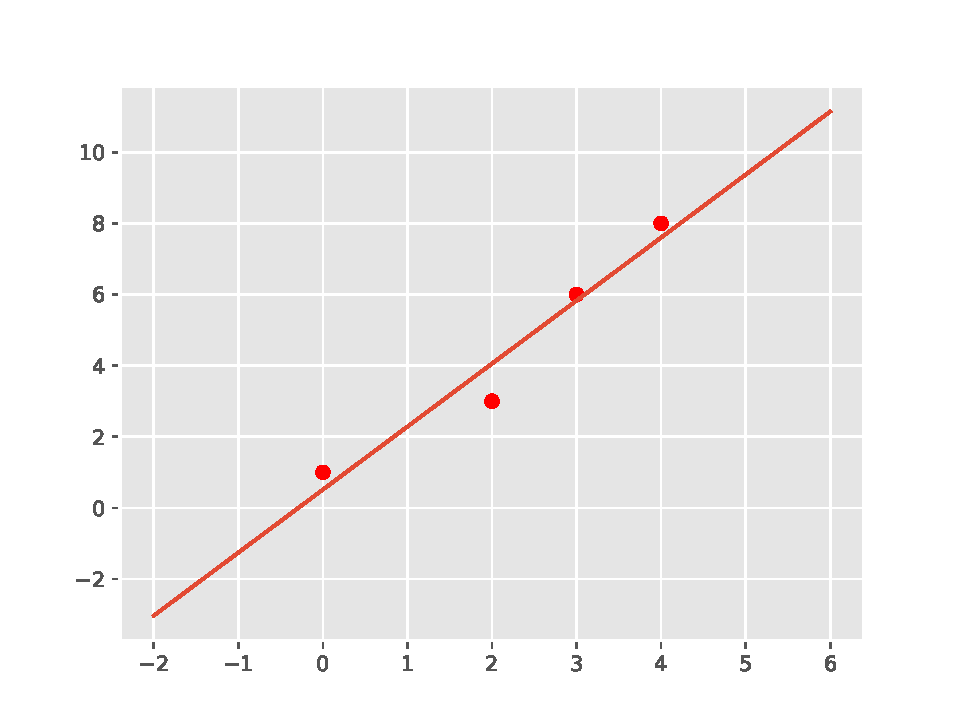
\includegraphics[width=8cm]{hw1pr2c.pdf}
        \caption{Optimal linear fit for $\mc{D}$}
      \end{figure}
    \item See plot below. The values for $m$ and $b$ were calculated
      to be
      \[
        m = 1.77377696 \qquad b = 0.40970185
      \]
      \begin{figure}[H]
        \centering
        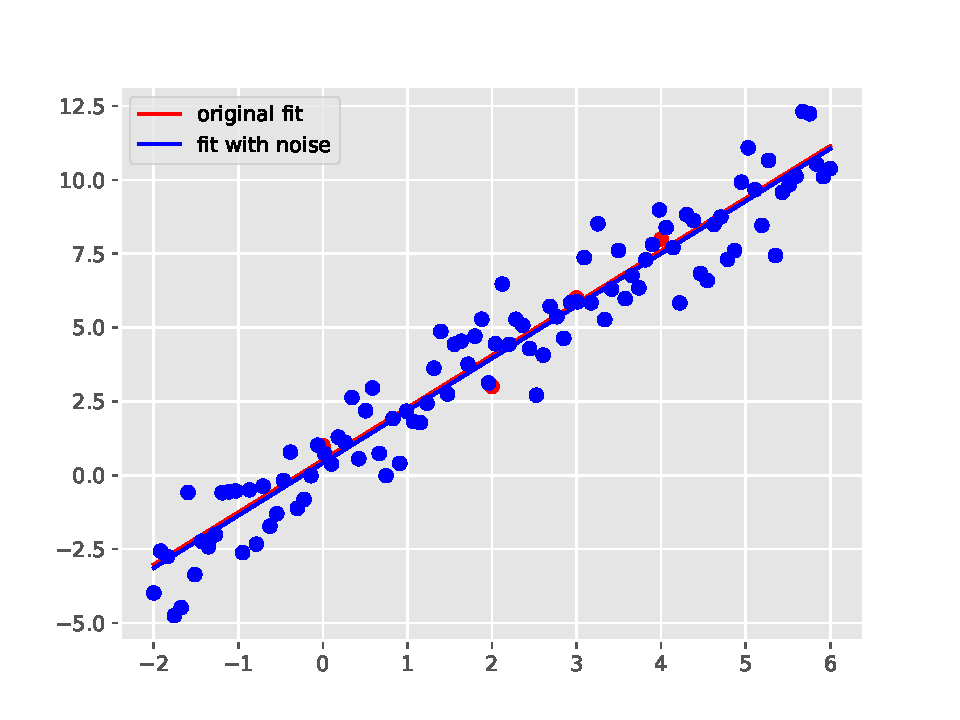
\includegraphics{hw1pr2d.pdf}
        \caption{Optimal linear fit for data with noise}
      \end{figure}
  \end{enumerate}

\end{document}
